
\documentclass[12pt]{article}

\usepackage{graphicx}
%\usepackage{subcaption}
\usepackage{amsmath}
\usepackage{amssymb}
%\usepackage{afterpage}
%\usepackage{showlabels}
% \usepackage{epstopdf}
% \usepackage{pdfpages}
\usepackage{geometry}
%\usepackage{wrapfig}
\usepackage{url}
\usepackage{times}
\usepackage{pdfpages}
\usepackage{etoolbox}
\usepackage{hyperref}
\usepackage{enumitem}
\hypersetup{
    colorlinks=true,
    linkcolor=blue,
    filecolor=magenta,
    urlcolor=cyan,
    pdftitle={Overleaf Example},
    pdfpagemode=FullScreen,
    }

\urlstyle{same}

\newcommand{\s}{\textrm{s}}
\newcommand{\m}{\textrm{m}}
\newcommand{\kg}{\textrm{kg}}
\newcommand{\N}{\textrm{N}}
\DeclareMathOperator{\sech}{sech}
\DeclareMathOperator{\arctanh}{arctanh}

\newcommand{\shortlist}{%
\parindent 0in%
\parskip   0in%
\itemsep   0in%
\topsep    0in%
\parsep    0in%
}

\setlength{\parindent}{0in}

\geometry{letterpaper,tmargin=1in,bmargin=1in,lmargin=1in,rmargin=1in}

\newcommand{\soln}[1] {\textit{Solution:} #1}

%\renewcommand{\soln}[1] {}

\newcommand{\Title}{PHYS 615 -- HW 5}

\begin{document}

\begin{center}
    {\Large\bfseries\Title}

\end{center}
\bigskip
\bigskip

\textbf{Types of homework questions}
\begin{itemize}\shortlist
    \item	RQ (Reading questions):  prompt you to go back to the text and read and think about the text more carefully and explain in your own words. While not directly tested in quizzes, can help you think more deeply about quiz questions.
    \item	BF (Building foundations):  gives you an opportunity to build and practice foundational skills that you have, presumably, seen before.
    \item	TQQ (typical quiz questions):   Similar questions (though perhaps longer or shorter) will be asked on quizzes.  But the difficulty level and skills tested will be similar.
    \item Design (D):  These are questions in which you are given a desired outcome and asked to figure out how to make it happen.  These will often also be TQQ’s, but always starting with desired motion/behavior as the given.
    \item	COMP (Computing): computing questions often related to TQQ but will never be asked on a quiz (since debugging can take so long).  You will need to do at least four computing questions over the semester
    \item	FC (free choice): allows you to decide where to put your time.  Any of the following are possible:  work through a section of the text or a lecture in detail; redo a problem from before; do an unassigned problem in the text; extend a computing project; try a problem using a different analytical approach (e.g. forces instead of conservation of energy).
    \item ACT (in-class activity): These questions are repeats of questions (or similar to) that occurred in a previous in-class activity.
    \item \textbf{Standard Reading Questions}: How does the reading connect with what you already know? What was something new?  Ask an "I wonder" question OR give an example applying the idea in the reading.
\end{itemize}

\textbf{Please remember to say something about the "Check/Learn" part at the end of solving a problem!}

Note that while this homework does not have designated "RQ" questions, in particular the activity-based questions can certainly benefit from reading the corresponding sections in the text.

Full credit will be given at 75\% of the total points possible, so you can choose a subset of problems (you can do more / all, but the score is capped at 75\%)

\begin{enumerate}
    \item TQQ / ACT (25 points) Hand in Activity 3.1 (except the challenge problem. You could use the challenge problem as your free choice problem.)

          \soln{See Activity 3.1 solution.}

    \item TQQ / ACT (20 points) Hand in Activity 3.2.

          \soln{See Activity 3.2 solution.}
    \item TQQ / ACT (15 points) Hand in Activity 3.3.

          \soln{See Activity 3.3 solution.}
    \item TQQ (10 points)

          A uniform thin sheet of metal is cut into the shape of a semicircle of radius $R$ and lies in the $x$-$y$ plane with its center at the origin and diameter along the $x$ axis. Find the position of the CM using polar coordinates. [In this case, Taylor's Eq. (3.9) becomes a two-dimensional integral of the form $\int \vec r \sigma dA$, where $\sigma$ denotes the surface mass density (mass / area) and $dA$ is the element of area $dA = r\,dr\,d\phi$.]

          \soln{The mass of the semicircle is $M = \sigma A = \sigma \frac{1}{2}\pi R^2$. The center of mass is given by
              $$
                  \vec R_{CM} = \frac{1}{M} \int_0^\pi d\phi \int_0^R dr \, r\sigma \vec r
              $$
              It is clear from symmetry that the center of mass is going to be located on the $y$ axis, ie., $x_CM = 0$, so I don't need to do the math for that. Since $y = r\sin\phi$:
              \begin{align*}
                  y_{CM} & = \frac{2}{\sigma \pi R^2} \int_0^\pi d\phi \int_0^R dr \, r\sigma r \sin\phi \\
                         & =\frac{2}{\pi R^2} \int_0^\pi d\phi \sin\phi \int_0^R dr\,r^2                 \\
                         & = \frac{2}{\pi R^2} (-\cos\phi)|_0^\pi \frac{1}{3}r^3|_0^R                    \\
                         & = \frac{2}{\pi R^2} 2 \frac{1}{3}R^3                                          \\
                         & = \frac{4}{3\pi}R \approx 0.42 R                                              \\
              \end{align*}
              That is below half-way up the $y$ axis, which makes sense.
          }


    \item TQQ (10 points)

          \begin{enumerate}
              \item
                    A vector $\vec a$ of magnitude $a = |\vec a|$ lies along the x direction. A second vector, $\vec b$ of magnitude $b$ is rotated counterclockwise from the $x$ axis by an angle of $\phi$. As we (hopefully) know, the direction of the cross product $\vec a \times \vec b$ is given by the right-hand rule, and the magnitude is $ab\sin \theta$, where $\theta$ is the angle between the two vectors.

                    Write down $\vec a \times \vec b$ using the above formula in vector components notation (ie., using components and unit vectors $\hat x, \hat y, \hat z$).

                    \soln{
                        My right middle finger points in the positive $z$ direction, and the angle between the two vectors happens to be just $\phi$ (or $180^\circ - \phi$, which leads to the same result).
                        $$\vec a \times \vec b = a b \sin\phi \hat z$$
                    }

                    Write down $\vec a$ and $\vec b$ individually in vector component notation.

                    \soln{$$\vec a = a \hat x\qquad \vec b = b \cos\phi \hat x + b \sin\phi \hat y$$}

                    Use the "determinant rule" to calculate the cross product. Does it match what you wrote down before? Does that meet your expectations? (See bottom of \url{https://betterexplained.com/articles/cross-product/} for calculating the cross product with the determinant, though it's probably what you usually use in any case.)

                    \soln{$$\vec a \times \vec b = 0\hat x + 0\hat y + ab\sin\phi\hat z$$

                        This the same as what I got before, and that is what I expected, since it's just another way of calculating the same thing -- the answer should be the same either way.
                    }
              \item
                    If the vectors $\vec a$ and $\vec b$ form two of the sides of a triangle, show that $\frac{1}{2}|\vec a \times \vec b|$ is equal to the area of that triangle.

                    \soln{The area of a triangle is one half base times height. If I consider $\vec a$ to be the base, I still have to find the height based on $b$ and the angle $\theta$ between $\vec a$ and $\vec b$. From the sketch, $h = b\sin\theta$, so $A = \frac{1}{2}ab\sin\theta$, which is $\frac{1}{2}|\vec a \times \vec b|$

                        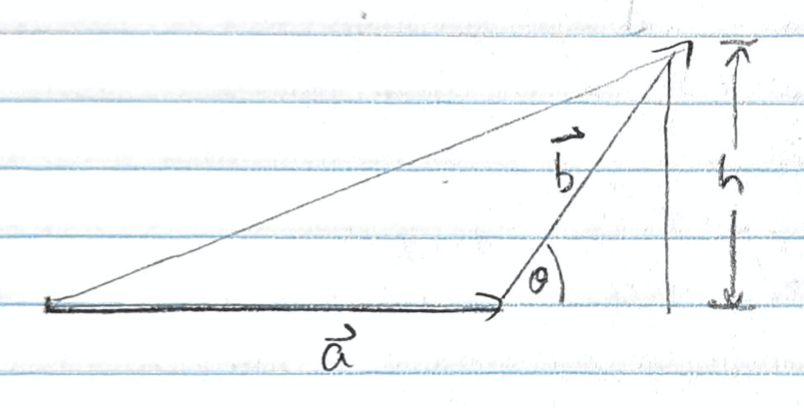
\includegraphics[width=.5\textwidth]{hw5_triangle.png}

                        Note that this also works if the angle is greater than $90^\circ$.
                    }

          \end{enumerate}

    \item RQ / TQQ (10 points)

          A particle moves under the influence of a central force directed toward a fixed origin $O$.
          \begin{enumerate}\item
                    Explain why the particle's angular momentum about $O$ is constant.

                    \soln{Angular momentum is changed by torque $\Gamma = \vec r \times \vec F$. Since a central force acts towards the center, ie., $\vec F = F\hat r$, that cross product is zero, so the change of angular momentum is zero, ie., it is conserved.}

              \item Give in detail Taylor's argument that the particle's orbit must lie in a single plane containing $O$.

                    \soln{Since angular momentum is conserved, $\vec l = \vec r \times \vec p$ remains constant, ie., $\vec r$ is always perpendicular to that constant $\vec l$. That means $\vec r$ lies in a plane perpendicular to $\vec l$ all throughout.}
          \end{enumerate}

    \item	FC (10 points) (free choice): allows you to decide where to put your time.  Any of the following are possible: work through a section of the text or a lecture in detail; polish up a group work assignment from class; redo a problem from before; do an unassigned problem in the text; extend a computing project; try a problem using a different analytical approach (e.g. forces instead of conservation of energy).

\end{enumerate}

\end{document}
